\usepackage{amssymb}
\usetikzlibrary{calc}
\usetikzlibrary{shapes.geometric}
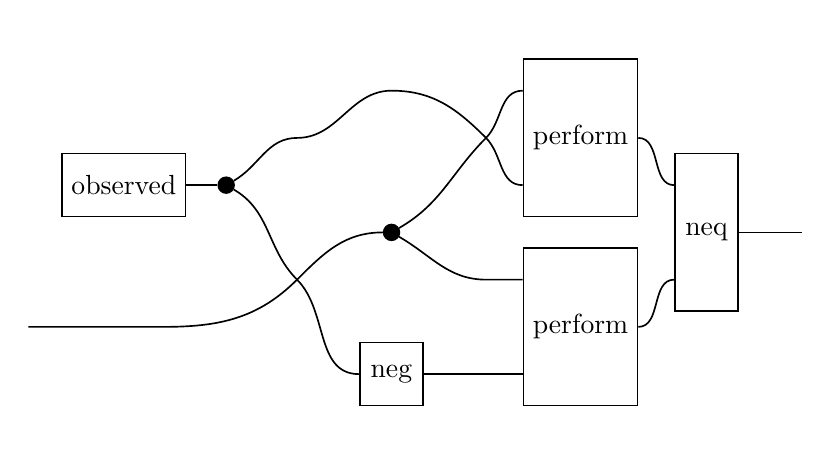
\begin{tikzpicture}[unit length/.code={{\newdimen\tikzunit}\setlength{\tikzunit}{#1}},unit length=4mm,x=\tikzunit,y=\tikzunit,semithick,box/.style={rectangle,draw,solid,sharp corners},junction/.style={circle,draw,fill,inner sep=0},outer box/.style={draw=none},wire/.style={draw}]
  \node[outer box,minimum width=24.5\tikzunit,minimum height=13\tikzunit] (root) at (0,0) {};
  \node[box,minimum size=2\tikzunit] (n3) at (-9.25,1.5) {$\mathrm{observed}$};
  \node[junction,minimum size=0.5\tikzunit] (n4) at (-6,1.5) {};
  \node[junction,minimum size=0.5\tikzunit] (n5) at (-0.75,0) {};
  \node[box,minimum size=2\tikzunit] (n6) at (-0.75,-4.5) {$\mathrm{neg}$};
  \node[box,minimum width=2\tikzunit,minimum height=5\tikzunit] (n7) at (5.25,3) {$\mathrm{perform}$};
  \node[box,minimum width=2\tikzunit,minimum height=5\tikzunit] (n8) at (5.25,-3) {$\mathrm{perform}$};
  \node[box,minimum width=2\tikzunit,minimum height=5\tikzunit] (n9) at (9.25,0) {$\mathrm{neq}$};
  \path[wire] ($(root.west)+(-0.0,-3)$) to[out=0,in=180] (-8,-3) to[out=0,in=-135] (-3.75,-1.5) to[out=45,in=180] (n5.180);
  \path[wire] (n3.east) to[out=0,in=180] (n4.180);
  \path[wire] (n4.-30) to[out=-30,in=135] (-3.75,-1.5) to[out=-45,in=-180] (n6.west);
  \path[wire] (n4.30) to[out=30,in=180] (-3.75,3) to[out=0,in=180] (-0.75,4.5) to[out=0,in=135] (2.25,3) to[out=-45,in=-180] ($(n7.west)+(0,-1.5)$);
  \path[wire] (n5.30) to[out=30,in=-135] (2.25,3) to[out=45,in=-180] ($(n7.west)+(0,1.5)$);
  \path[wire] (n5.-30) to[out=-30,in=180] (2.25,-1.5) to[out=0,in=-180] ($(n8.west)+(0,1.5)$);
  \path[wire] (n6.east) to[out=0,in=180] (2.25,-4.5) to[out=0,in=-180] ($(n8.west)+(0,-1.5)$);
  \path[wire] (n7.east) to[out=0,in=-180] ($(n9.west)+(0,1.5)$);
  \path[wire] (n8.east) to[out=0,in=-180] ($(n9.west)+(0,-1.5)$);
  \path[wire] (n9.east) to[out=0,in=180] (root.east);
\end{tikzpicture}